\section{Many agents over time}\label{sec:collective}

The brain was built to let agents work together across time: an agent today should be able to stand on what an agent did last month without either of them knowing the other existed. We describe the arrangements that made this possible and then the record of the store's growth, which is the best evidence we have that it happened.

\subsection{How the agents shared work}
Three kinds of agents wrote to the store.
\begin{enumerate}[label=(\alph*)]
\item \emph{Interactive agents} of two runtimes (Claude Code and Codex) working with the author on particular problems. These register in a coordination mesh, claim the files and topics they will change, and release them when done, so that two agents do not write the same result twice.
\item \emph{Fleets} of headless agents launched on one problem or one list of problems, each with its own session, a common work order and a shared folder for reports. Up to a hundred agents worked one conjecture in parallel.
\item \emph{Scheduled tasks}: ChatGPT tasks that run every hour, read a common board (an owner message, a mode, a queue and a roster), do one unit of work, and commit a report to a shared repository. The board is edited only by the author; every task reads it at every run, so a change of direction reaches all of them within the hour.
\end{enumerate}
Reports from fleets and scheduled tasks enter the store the same way an interactive agent's results do: someone turns them into a packet, and the packet passes the gates of Section~\ref{sec:writeback}. A work order states the target, what is already known (by card identifiers), what is ruled out, and what counts as progress; on the Fourier entropy-influence campaign, for example, the order of 12 October assigned every scheduled worker to one dimension-free theorem and required each report to record the precise new result, its proof or reproducible counterexample, and the next unpaid step.

\subsection{Growth}
Figure~\ref{fig:growth} shows the number of cards and links from 2 August to 22 October 2026. The store grew in two ways. Large steps are harvests: on 30 August ($2{,}000$ cards), 2 September ($1{,}194$) and 7 September ($2{,}427$ cards, $1{,}993$ links) whole bodies of literature were turned into cards, and on 7 October a linking pass wrote $8{,}822$ links, mostly dependencies ($4{,}316$) and citations ($3{,}344$). Between the steps, growth is the agents' own work: on 10 October $1{,}103$ cards and $1{,}314$ links from $231$ packets, and on 21 October $921$ cards and $450$ links from $463$ packets, most of them results of the open-problem campaigns. Appendix~\ref{app:tables} gives the day-by-day record.

\begin{figure}[ht]
\centering
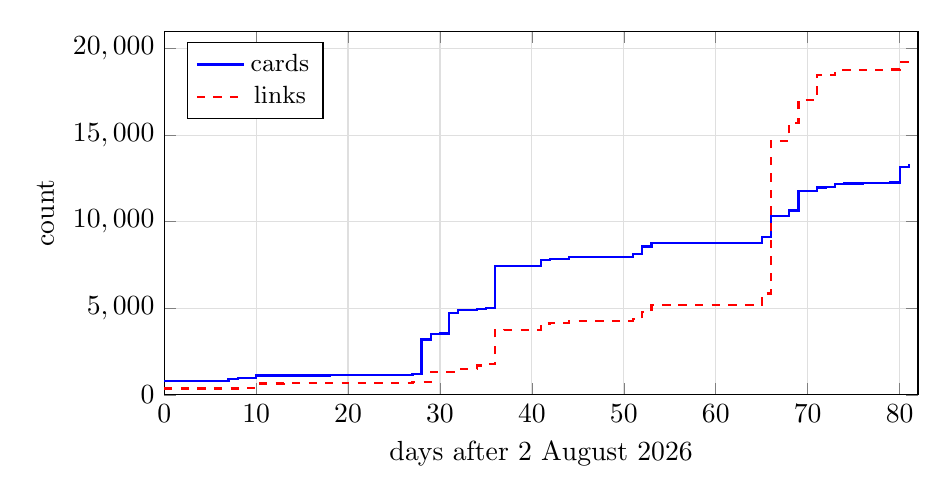
\begin{tikzpicture}
\begin{axis}[
  width=0.92\textwidth, height=6.2cm,
  xlabel={days after 2 August 2026}, ylabel={count},
  xmin=0, xmax=82, ymin=0, ymax=21000,
  legend pos=north west, legend style={font=\small},
  scaled y ticks=false, yticklabel style={/pgf/number format/fixed,/pgf/number format/1000 sep={,}},
  grid=major, grid style={gray!25}]
\addplot[thick, blue, const plot] coordinates {
(0,800)(7,924)(8,958)(10,1114)(13,1121)(18,1131)(20,1155)(27,1191)(28,3191)(29,3526)(30,3538)(31,4732)(32,4895)(34,4970)(35,5006)(36,7433)(37,7443)(38,7450)(40,7451)(41,7803)(42,7865)(44,7947)(49,7975)(51,8114)(52,8568)(53,8772)(54,8776)(55,8776)(59,8778)(64,8785)(65,9105)(66,10319)(68,10650)(69,11753)(71,11979)(72,11982)(73,12188)(74,12200)(75,12207)(76,12213)(77,12245)(78,12247)(79,12257)(80,13178)(81,13306)};
\addlegendentry{cards}
\addplot[thick, red, dashed, const plot] coordinates {
(0,372)(7,372)(8,379)(10,654)(13,663)(18,670)(20,703)(27,735)(28,735)(29,1332)(30,1337)(31,1337)(32,1507)(34,1697)(35,1760)(36,3753)(37,3761)(38,3765)(40,3766)(41,4124)(42,4162)(44,4244)(49,4269)(51,4362)(52,4798)(53,5176)(54,5188)(55,5194)(59,5195)(64,5207)(65,5853)(66,14675)(68,15712)(69,17026)(71,18458)(72,18477)(73,18740)(74,18749)(75,18753)(76,18757)(77,18773)(78,18774)(79,18782)(80,19232)(81,19362)};
\addlegendentry{links}
\end{axis}
\end{tikzpicture}
\caption{Cumulative cards and links (retracted links included), 2 August to 22 October 2026 (day $0$ is 2 August). Steps on days $28$, $31$ and $36$ are harvests of the literature; the step in links on day $66$ (7 October) is a linking pass over existing cards.}
\label{fig:growth}
\end{figure}

\subsection{Links across time}
If agents only ever linked a new card to cards written in the same session, the store would be a set of disconnected notebooks. The record says otherwise. For each link we compare the days on which its two endpoints were created. Of the $19{,}362$ links (the $231$ retracted ones included, about one percent), $12{,}267$ ($63\%$) join cards created on different days, and $9{,}164$ ($47\%$) join cards created thirty or more days apart (Table~\ref{tab:lag}). For dependencies the figure is $4{,}038$ of $9{,}129$, but most of these were written in one pass: on 7 October a linking campaign joined existing cards to the lemmas they use and wrote $3{,}469$ of them. The remaining $569$, written on other days, are the ones that record the intended pattern, a result written in October that uses a lemma written in August while the result was being written.

\begin{table}[ht]
\centering\small
\begin{tabular}{lrrrrr}
\toprule
Kind & same day & 1--6 days & 7--29 days & 30+ days & added after both endpoints\\
\midrule
\texttt{depends\_on} & 3{,}786 & 595 & 710 & 4{,}038 & 667\\
\texttt{cites} & -- & -- & -- & 3{,}603 & --\\
\texttt{analogous\_to} & -- & -- & -- & -- & 300 of 604\\
\texttt{fails\_under} & -- & -- & -- & -- & 114 of 160\\
\midrule
all kinds & 7{,}095 & 1{,}623 & 1{,}480 & 9{,}164 & \\
\bottomrule
\end{tabular}
\caption{The gap in days between the creation of a link's two endpoints. The last column counts links created on a day later than both endpoints: a relation noticed after both results were written. Entries marked -- are not broken out.}
\label{tab:lag}
\end{table}

Two caveats apply to this table. Some long-gap links are automatic: a \texttt{supersedes} link joins a revision to an older one by construction, and a \texttt{cites} link from a new result to an old source says only that the source was in the store; the \texttt{semantic\_association} links are written by a vocabulary pass. The figures that reflect agents working across time are the dependencies with long gaps, the analogies added after both endpoints ($300$ of $604$), and the pitfalls added after both endpoints ($114$ of $160$): in each case an agent noticed a relation between results it had not written.

The table is evidence that work accumulated; it is not a controlled measurement that accumulation helped. A controlled test of a fleet with a shared memory against the same fleet without one, on problems neither has seen, is the subject of Section~\ref{sec:campaign}. The one such comparison we have, on thirteen new open problems, did not favour the brain (Section~\ref{sec:tests}), and we discuss why.

\subsection{What the agents did with it}
The clearest examples are in Section~\ref{sec:math}. On the Fourier entropy-influence conjecture the agents' results on particular classes (the classes on which the inequality was proved with explicit constants, and the routes that failed) were written as cards, linked to the definitions and to each other, and read by later fleets; the reduction proved in Section~\ref{sec:math} was found by a fleet that started from those cards, and its first numerical evidence came from routes recorded as refuted. A card recording a refuted route is cheap to write and saves every later agent the cost of refuting it again; on that campaign the store holds the refutation of a selection lemma at one parameter value and its survival, still open, at another.
